24. \begin{figure}[ht!]
\center{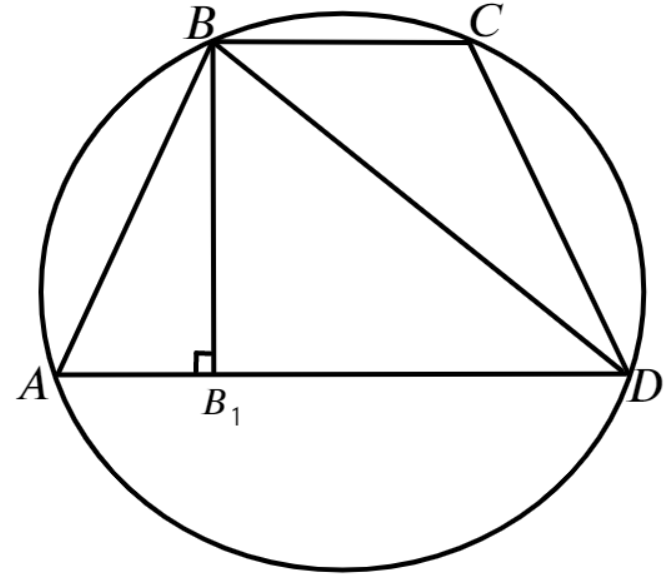
\includegraphics[scale=0.35]{g9-22.png}}
\end{figure}\\
Если трапеция является вписанной, то она равнобедренная. Если трапеция является описанной, то суммы её противоположных сторон равны, значит боковая сторона трапеции равна $\cfrac{2+14}{2}=8$см. Опустим высоту $BB_1,$ тогда $BB_1=2\cdot4=8$см, так как высота трапеции равна диаметру вписанной окружности. В таком случае высота трапеции оказалась равна её боковой стороне, что невозможно (в этом случае трапеция становится прямоугольником). Значит, трапеции с заданными параметрами не существует.\\
